\documentclass{article}

\usepackage{hyperref}
\hypersetup{
	colorlinks=true,
	linkcolor=blue,
	urlcolor=cyan,}
\usepackage{booktabs}
\usepackage{textgreek}

%%%%%%%%%%%%%%%%%%%%%%%%%%%%%%%%%%%%%%%%%
% Lachaise Assignment
% Structure Specification File
% Version 1.0 (26/6/2018)
%
% This template originates from:
% http://www.LaTeXTemplates.com
%
% Authors:
% Marion Lachaise & François Févotte
% Vel (vel@LaTeXTemplates.com)
%
% License:
% CC BY-NC-SA 3.0 (http://creativecommons.org/licenses/by-nc-sa/3.0/)
% 
%%%%%%%%%%%%%%%%%%%%%%%%%%%%%%%%%%%%%%%%%

%----------------------------------------------------------------------------------------
%	PACKAGES AND OTHER DOCUMENT CONFIGURATIONS
%----------------------------------------------------------------------------------------

\usepackage{amsmath,amsfonts,stmaryrd,amssymb} % Math packages

\usepackage{enumerate} % Custom item numbers for enumerations

\usepackage[ruled]{algorithm2e} % Algorithms

\usepackage[framemethod=tikz]{mdframed} % Allows defining custom boxed/framed environments

\usepackage{listings} % File listings, with syntax highlighting
\lstset{
	basicstyle=\ttfamily, % Typeset listings in monospace font
}

%----------------------------------------------------------------------------------------
%	DOCUMENT MARGINS
%----------------------------------------------------------------------------------------

\usepackage{geometry} % Required for adjusting page dimensions and margins

\geometry{
	paper=a4paper, % Paper size, change to letterpaper for US letter size
	top=2.5cm, % Top margin
	bottom=3cm, % Bottom margin
	left=2.5cm, % Left margin
	right=2.5cm, % Right margin
	headheight=14pt, % Header height
	footskip=1.5cm, % Space from the bottom margin to the baseline of the footer
	headsep=1.2cm, % Space from the top margin to the baseline of the header
	%showframe, % Uncomment to show how the type block is set on the page
}

%----------------------------------------------------------------------------------------
%	FONTS
%----------------------------------------------------------------------------------------

\usepackage[utf8]{inputenc} % Required for inputting international characters
\usepackage[T1]{fontenc} % Output font encoding for international characters

\usepackage{XCharter} % Use the XCharter fonts

%----------------------------------------------------------------------------------------
%	COMMAND LINE ENVIRONMENT
%----------------------------------------------------------------------------------------

% Usage:
% \begin{commandline}
%	\begin{verbatim}
%		$ ls
%		
%		Applications	Desktop	...
%	\end{verbatim}
% \end{commandline}

\mdfdefinestyle{commandline}{
	leftmargin=10pt,
	rightmargin=10pt,
	innerleftmargin=15pt,
	middlelinecolor=black!50!white,
	middlelinewidth=2pt,
	frametitlerule=false,
	backgroundcolor=black!5!white,
	frametitle={Command Line},
	frametitlefont={\normalfont\sffamily\color{white}\hspace{-1em}},
	frametitlebackgroundcolor=black!50!white,
	nobreak,
}

% Define a custom environment for command-line snapshots
\newenvironment{commandline}{
	\medskip
	\begin{mdframed}[style=commandline]
}{
	\end{mdframed}
	\medskip
}

%----------------------------------------------------------------------------------------
%	FILE CONTENTS ENVIRONMENT
%----------------------------------------------------------------------------------------

% Usage:
% \begin{file}[optional filename, defaults to "File"]
%	File contents, for example, with a listings environment
% \end{file}

\mdfdefinestyle{file}{
	innertopmargin=1.6\baselineskip,
	innerbottommargin=0.8\baselineskip,
	topline=false, bottomline=false,
	leftline=false, rightline=false,
	leftmargin=2cm,
	rightmargin=2cm,
	singleextra={%
		\draw[fill=black!10!white](P)++(0,-1.2em)rectangle(P-|O);
		\node[anchor=north west]
		at(P-|O){\ttfamily\mdfilename};
		%
		\def\l{3em}
		\draw(O-|P)++(-\l,0)--++(\l,\l)--(P)--(P-|O)--(O)--cycle;
		\draw(O-|P)++(-\l,0)--++(0,\l)--++(\l,0);
	},
	nobreak,
}

% Define a custom environment for file contents
\newenvironment{file}[1][File]{ % Set the default filename to "File"
	\medskip
	\newcommand{\mdfilename}{#1}
	\begin{mdframed}[style=file]
}{
	\end{mdframed}
	\medskip
}

%----------------------------------------------------------------------------------------
%	NUMBERED QUESTIONS ENVIRONMENT
%----------------------------------------------------------------------------------------

% Usage:
% \begin{question}[optional title]
%	Question contents
% \end{question}

\mdfdefinestyle{question}{
	innertopmargin=1.2\baselineskip,
	innerbottommargin=0.8\baselineskip,
	roundcorner=5pt,
	nobreak,
	singleextra={%
		\draw(P-|O)node[xshift=1em,anchor=west,fill=white,draw,rounded corners=5pt]{%
		Question \theQuestion\questionTitle};
	},
}

\newcounter{Question} % Stores the current question number that gets iterated with each new question

% Define a custom environment for numbered questions
\newenvironment{question}[1][\unskip]{
	\bigskip
	\stepcounter{Question}
	\newcommand{\questionTitle}{~#1}
	\begin{mdframed}[style=question]
}{
	\end{mdframed}
	\medskip
}

%----------------------------------------------------------------------------------------
%	WARNING TEXT ENVIRONMENT
%----------------------------------------------------------------------------------------

% Usage:
% \begin{warn}[optional title, defaults to "Warning:"]
%	Contents
% \end{warn}

\mdfdefinestyle{warning}{
	topline=false, bottomline=false,
	leftline=false, rightline=false,
	nobreak,
	singleextra={%
		\draw(P-|O)++(-0.5em,0)node(tmp1){};
		\draw(P-|O)++(0.5em,0)node(tmp2){};
		\fill[black,rotate around={45:(P-|O)}](tmp1)rectangle(tmp2);
		\node at(P-|O){\color{white}\scriptsize\bf !};
		\draw[very thick](P-|O)++(0,-1em)--(O);%--(O-|P);
	}
}

% Define a custom environment for warning text
\newenvironment{warn}[1][Warning:]{ % Set the default warning to "Warning:"
	\medskip
	\begin{mdframed}[style=warning]
		\noindent{\textbf{#1}}
}{
	\end{mdframed}
}

%----------------------------------------------------------------------------------------
%	INFORMATION ENVIRONMENT
%----------------------------------------------------------------------------------------

% Usage:
% \begin{info}[optional title, defaults to "Info:"]
% 	contents
% 	\end{info}

\mdfdefinestyle{info}{%
	topline=false, bottomline=false,
	leftline=false, rightline=false,
	nobreak,
	singleextra={%
		\fill[black](P-|O)circle[radius=0.4em];
		\node at(P-|O){\color{white}\scriptsize\bf i};
		\draw[very thick](P-|O)++(0,-0.8em)--(O);%--(O-|P);
	}
}

% Define a custom environment for information
\newenvironment{info}[1][Info:]{ % Set the default title to "Info:"
	\medskip
	\begin{mdframed}[style=info]
		\noindent{\textbf{#1}}
}{
	\end{mdframed}
}
 % Include the file specifying the document structure and custom commands

%----------------------------------------------------------------------------------------
%	ASSIGNMENT INFORMATION
%----------------------------------------------------------------------------------------

\title{Week 7: Blood Pressure (BP)}
\author{BIOE 320 Systems Physiology Laboratory} 
\date{}
%----------------------------------------------------------------------------------------

\begin{document}
\large
\maketitle

\section*{Objectives}
\begin{enumerate}
	\item To become familiar with auscultatory methods of measuring arterial blood pressure, using the appearance and disappearance of Korotkoff sounds to identify systolic and diastolic pressures.
	\item To measure and compare system arterial blood pressure in an individual's left arm and right arm under identical environmental conditions.
	\item To use measured values of systolic and diastolic blood pressure to compute and compare pulse pressure and mean arterial pressure under different experimental conditions.
	\item To compute pulse pressure wave velocity using the time difference between the peak of the R wave of the ECG and the occurrence of the first Korotkoff sound.
\end{enumerate}

\section*{Background}

\begin{figure}[h]
\centering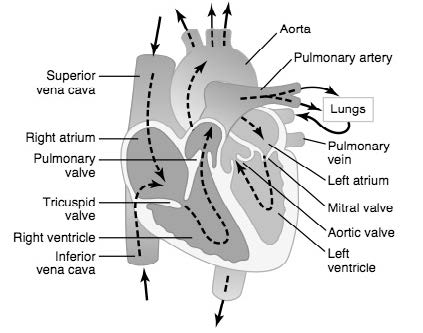
\includegraphics[width=0.5\textwidth]{../images/BP_1.jpg}
\caption{Blood flow through the heart chambers}
\label{flow}
\end{figure}

The heart circulates blood throughout the body to deliver oxygen, nutrients, and various compounds to the surrounding tissue. As the heart pumps, blood is cycled through the entire body in a unidirectional process. As shown in Fig. \ref{flow}, blood enters the right atrium of the heart through the superior and inferior vena cava. The blood flows through the tricuspid valve to the right ventricle and out of the heart via the pulmonary artery to the lungs. The now oxygenated blood returns to the heart by way of the pulmonary vein. The blood then travels into the left atrium, through the mitral valve, and into the left ventricle, from where it is pumped via the aorta back into systemic circulation.\\

The contraction of the ventricles is called \textbf{ventricular systole}. During systole, the atrioventricular valves (tricuspid and mitral valves) close to prevent back flow of blood into the atria, whereas the semilunar valves (pulmonary and aortic valves) open to allow blood to leave the ventricles. The relaxation of ventricles is called \textbf{ventricular diastole}. During diastole, the atrioventricular valves open, allowing blood to flow from the atria into the ventricles, whereas the semilunar valves are closed to prevent blood from leaving the ventricles.\\

As the blood travels through the circulatory system, it exerts pressure on the vessel walls. This force of blood pushing against the walls of the arteries is known as blood pressure. Several key factors influence the measurement of blood pressure, such as: stroke volume, resistance of blood vessel, viscosity of blood. Since the ventricles alternate between systole and diastole, the arterial blood pressure and associated blood flow are \textbf{pulsatile}. Blood pressure is higher during systole and lower during diastole (Fig. \ref{systole}).

\begin{figure}[h]
\centering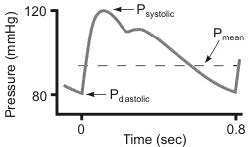
\includegraphics[width=0.5\textwidth]{../images/BP_2.jpg}
\caption{Arterial blood pressure over time}
\label{systole}
\end{figure}

\textbf{Systolic pressure} is the force of blood against the arterial walls during ventricular contraction. It is the highest value reached during ventricular contraction and is typically less than 120 mmHg. \textbf{Diastolic pressure} is the lowest arterial pressure reached during ventricular relaxation. It is measured at the end of diastole when the relaxation of the ventricles is the greatest. Normal diastolic pressure values are less than 80 mmHg. \textbf{Pulse pressure} is a measure of the force that travels through the circulatory system and can be calculated as the difference between the diastolic and systolic pressures. The \textbf{mean arterial pressure} (MAP) is a weighted average of systolic and diastolic pressures, and can be calculated as: $(P_{systolic} + 2P_{diastolic})/3$.\\

The most common way to measure arterial pressure is the auscultatory method. A blood pressure cuff with an attached pressure gauge is wrapped around the arm and inflated to collapse the underlying artery (commonly the brachial artery for adults). A stethoscope is placed over the collapsed artery to listen to blood flow (Fig. \ref{method}).

\begin{figure}[h]
\centering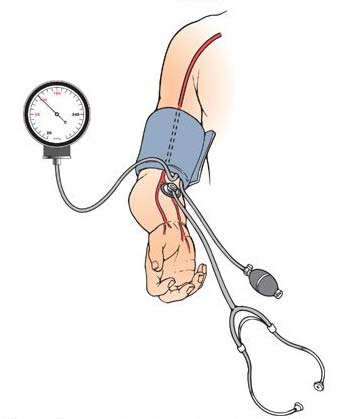
\includegraphics[width=0.4\textwidth]{../images/BP_3.jpg}
\caption{Auscultatory method for measuring systolic and diastolic arterial pressures}
\label{method}
\end{figure}

The sounds picked up the stethoscope are known as Korotkoff sounds. The first Korotkoff sound is a sharp tapping sound that is heard when the pressure in the cuff equals the systolic blood pressure. This is the point at which blood can turbulently flow through the squeezed artery. The next three Korotkoff sounds are knocking, whooshing, and muffling. The fifth "sound" is silence. The transition from muffling to silence represents diastolic pressure. This is the pressure at which the artery is no longer squeezed and blood resumes laminar flow (Fig. \ref{sounds}). To obtain the most accurate results when measuring blood pressure, the subject should sit with arms at heart level and should not have consumed tobacco or caffeine within the last 30 minutes. Make sure the cuff fits snug around the arm to avoid erroneous readings.

\begin{figure}[h]
\centering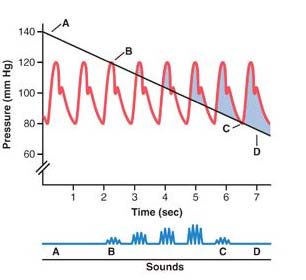
\includegraphics[width=0.4\textwidth]{../images/BP_4.jpg}
\caption{Systolic and diastolic arterial pressures and Korotkoff sounds}
\label{sounds}
\end{figure}

\section*{Experimental Methods}
In this lab, you will use Korotkoff sounds to measure systolic and diastolic arterial pressure, then use these values to compute pulse pressure and mean arterial pressure. You will perform these measurements against several different experimental conditions, including the subject's right arm vs. left arm, sitting up, lying down, and after exercise.

\subsection*{Hardware and Software Setup}
\begin{enumerate}
	\item Open the BIOPAC Lab PRO software (NOT BIOPAC student lessons).
	\item Plug the blood pressure cuff into channel 1 of the MP3X unit.
	\item Plug the stethoscope into channel 2.
	\item Plug the ECG leads into channel 3.
	\item Connect your ECG lead to measure standard bipolar lead II as follows:\begin{itemize}
		\item Red (+): left leg
		\item White (-): right arm
		\item Black (ground): right ankle
	\end{itemize}
	\item Turn the MP3X unit on.
	\item Go to the MP3X pull down menu and select Setup Channels.
	\begin{enumerate}
		\item Check all the boxes for channels 1, 2, and 3 (Fig. \ref{setup}).
		\item Click on presets and set each channel to:\begin{itemize}
			\item channel 1: blood pressure cuff
			\item channel 2: stethoscope
			\item channel 3: ECG (0.5 to 150 Hz)
		\end{itemize}
	\end{enumerate}
\end{enumerate}

\begin{figure}[h]
\centering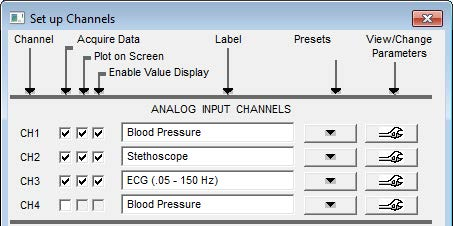
\includegraphics[width=0.6\textwidth]{../images/BP_5.jpg}
\caption{Setup channels menu}
\label{setup}
\end{figure}

\subsection*{Calibrate Blood Pressure Cuff}
\begin{enumerate}
	\item Under Setup Channels, click on the wrench to the right of channel 1 (blood pressure).
	\item A new menu should appear, click on scaling at the bottom of the menu.
	\item Deflate the cuff completely by loosening the screw attached to the sphygmomanometer so that it displays 0 mmHg. Make sure the subject is not connected to the pressure cuff.
	\item Click on Cal1, the input value should now be a value close to 0 mV.
	\item Tighten the screw to close the valve and pump to inflate the cuff to 100 mmHg.
	\item Click on Cal2, the input value should now be a value close to 2.5 mV.
\end{enumerate}

\subsection*{Acquisition Setup}
\begin{enumerate}
	\item Go to the MP3X pull down menu and select Setup Acquistion.
		\item Set Sample to 2000 samples/sec.
		\item Set Acquisition Length to 60 minutes.
		\item Close the box.
\end{enumerate}

\subsection*{Measuring Systolic and Diastolic Blood Pressures}
We will be using the stethoscope to listen for Korotkoff sounds at the brachial artery, which will allow us to determine the systolic and diastolic blood pressures. Because finding the brachial artery and properly adjusting the pressure of the cuff can be tricky, we will begin with a warm up trial.

\begin{warn}
	Do not use pressures over 140 mmHg, and do not keep pressure applied for over a minute, as permanent damage could be caused by excessive pressure or a sustained time of blood flow loss to the extremities. If you feel nauseous or light-headed, immediately release the pressure cuff and alert the instructor.
\end{warn}

\subsubsection*{Warm Up Trial}
\begin{enumerate}
	\item The subject needs to make the left brachial artery accessible by removing any jackets or heavy clothes, then rolling up their left sleeve.
	\item Using alcohol wipes, clean the stethoscope's earpieces and diaphragm.
	\item Wrap the blood pressure cuff around the left arm above the elbow and place the stethoscope on the brachial artery (inside the pressure cuff). See Fig. \ref{setup_2} for an example.
		\begin{figure}[h]
		\centering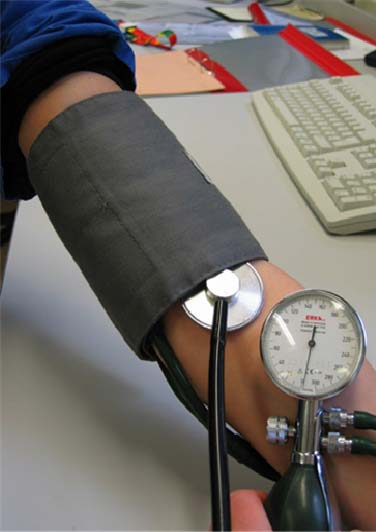
\includegraphics[width=0.4\textwidth]{../images/BP_6.jpg}
		\caption{Correct setup for measurements}
		\label{setup_2}
		\end{figure}
		
	\item Have the stethoscope ready, and tighten the screw on the sphygmomanometer to close off the valve (air should not be leaking out of the pressure cuff).
	\item Start recording with BIOPAC.
	\item Inflate the cuff to 140 mmHg, then slowly release pressure at a rate of about 3-5 mmHg per second while listening for Korotkoff sounds.
	\begin{info}
		You may need to move the stethoscope microphone to find the brachial artery. Once you find the spot, mark it with a pen so you don't lose it!
	\end{info}
	
	\item When you begin to hear Korotkoff sounds, create a marker for systolic pressure. Try to listen for different types of Korotkoff sounds (you do not need to note these with a marker).
	\item When you no longer hear Korotkoff sounds, create another marker for diastolic pressure.
	\item Do not stop recording or fully deflate the cuff after you hear the diastolic pressure. Keep deflating the cuff at the same rate for 5-10 more seconds.
	\item Stop recording.
	\item Check your data to make sure that:\begin{itemize}
		\item The markers are showing up.
		\item The ECG looks correct.
		\item The stethoscope data shows spikes that represent the Korotkoff sounds.
	\end{itemize}
\end{enumerate}

You may need to repeat this trial a few times to get the hang of it, but make sure the subject has time to rest between trials. Remember you should not keep pressure on the cuff for more than 1 minute at a time.

\subsubsection*{Measuring Under Different Conditions}
Now that you feel confident measuring blood pressure using the stethoscope and pressure cuff, you will record a series of trials under different scenarios.
\begin{enumerate}
	\item There will be 4 segments that you will be recording systolic and diastolic pressure through the auscultatory method.\begin{itemize}
		\item Segment 1: left arm, while sitting up
		\item Segment 2: right arm, while sitting up
		\item Segment 3: right arm, while lying down
		\item Segment 4: right arm, immediately after exercise
	\end{itemize}
	\item These trials will be conducted similarly to the warm up trial (follow the steps in the previous section).
	\item Repeat the trial steps for each of the conditions twice, as we will use the average of these two systolic and diastolic pressure values for our calculations. Record your values in the tables in the handout.
\end{enumerate}

\section*{Data Analysis}
\begin{enumerate}
	\item Give one reason why blood pressure in the left arm may be different than blood pressure in the right arm for the sitting up condition.
	\item Using the ECG data, calculate the beats per minute (BPM) for the four conditions measured
	\item Calculate mean arterial pressure (MAP) and pulse pressure for the four conditions measured.
	\item Determine the time delay from the peak of an R wave to the beginning of a sound. This requires zooming into a section so that individual waves can be seen.
	\item What is this time delay a measure of?
	\item We will now estimate the distance travelled by the pulse wave, by measuring the length from the sternum to the antecubital fossa and use that value to calculate the pulse speed. Use the right arm, sitting up data for these calculations.
	\item How does the speed of the pulse wave calculated here compare with published values?
	\item Does your systolic and/or diastolic arterial pressure change as your heart rate increases? How does this change affect your pulse pressure?
	\item Name another artery other than the brachial that could be used for an indirect measurement of blood pressure and explain your choice.
\end{enumerate}
\end{document}
